\chapter{Introduction}

\pagenumbering{arabic}
\setcounter{page}{1}
\graphicspath{{images/}}
Robotic systems are used to enhance even the most mundane aspects of daily life. Robots can clean our floors, dispense our soft drinks, and, pretty soon, drive us around town. Powerful and precise, robots are also used to make up for the qualities humans lack. They can do and see what humans cannot, and are resilient in situations where humans physically could not be. As one might imagine, robots are used to perform great feats. 

	Recently, autonomous systems have been of great interest to robotics experts. The race to fully autonomous driving is at its peak with GM, Mercedes-Benz, Audi, Nissan, BMW, Renault, Tesla and Google all expecting to sell at least partially autonomous vehicles by 2020\cite{autonomouscars}; however, the applications for autonomous systems are expanding past commercial uses. Researchers are now looking to use unmanned and partially autonomous vehicles, both ground and air, to aid in providing relief services in the event of a natural disaster.\cite{dronesrescueservices}
    
	Gathering information is a critical part of providing disaster relief services.  This is true both immediately following a natural disaster, and for prolonged periods of time afterwards.  Relief service personnel and investigators place themselves in dangerous environments in order to assist those affected by a natural disaster.  To avoid placing human lives in unnecessary danger, relief services have begun to rely on unmanned vehicles to gather information. 
    
	Drones, in particular, have been utilized to collect this information; however, the environment after a natural disaster is not always conducive to drone activity.  Extreme weather, dust, and smoke are all conditions that make it difficult for drones to operate and gather information to aid relief services \cite{aerialsupervisionguide}.  In certain situations like wildfires, having drones in the air actually severely impacts the ability of firefighters to combat wildfires.  While a drone is in the air, other manned aerial vehicles cannot enter the airspace, preventing them from performing vital operations \cite{firedrones}.

Furthermore, the area after the initial relief service efforts can remain hostile for indefinite periods of time.  Investigators looking to determine the root cause of a disaster -- building collapse, wildfire, flood, etc. -- have to be aware of:
\begin{itemize}
  \item building structural integrity
  \item smoke
  \item electrical, chemical, or biological hazards
  \item other health risks \cite{firearsonsceneevidence}.
\end{itemize}   This investigatory period can be as dangerous as the initial relief service operations. This poses the question: how can robots be used to allow post-disaster investigators to safely determine what types of risks lurk within the disaster zone?

\section{Motivation}
The motivation behind our project has been to provide an unmanned vehicle that can examine an environment after a natural disaster so that humans do not have to place their lives in danger to do so. 
\begin{itemize}
\item Santa Clara University possesses a 2004 Series 11 Polaris Ranger 6x6 that is ideal for traversing a rugged environment. (See Figure ~\ref{fig:rover3fig} on page ~\pageref{fig:rover3fig})
\item Members of our team have personal relationships with those who serve as fire responders.
\item Other members have access to the types of sensors and testing locations that would be ideal to implement a vehicle that can aid in any post-fire investigation efforts.
\end{itemize} 
So, we were motivated to design an unmanned vehicle that can specifically examine a post-fire environment and ultimately keep fire responders out of hazardous situations.

\begin{figure}[H]
\centering
\includegraphics[scale=0.15]{rover3}
\caption{Polaris 6x6 Ranger}
\label{fig:rover3fig}
\end{figure}

\section{Literature Review}
The sources reviewed have revealed a need for an unmanned vehicle that can assess the hazards, particularly pertaining to air quality, that lurk in a post-fire environment. "Guide for fire and explosion investigations" by the National Fire Protection Association gave a detailed procedure that fire responders follow while investigating the cause and damage of a fire\cite{nfpa} and "Evaluation of hazards in the post-fire environment" by The Interagency Board revealed the specific risks fire responders are exposed to while investigating a fire\cite{evaluationofhazards}. More information can be found in the remainder of this section. These two sources in particular helped inspire and shape the functionality of our vehicle and provided the motivation behind using an unmanned vehicle to assess a post-fire environment. There is a need for an unmanned vehicle that can help determine whether a post-fire zone is dangerous for fire servicemen, law enforcement officers, and various other people to enter, even with protective clothing and masks.\cite{evaluationofhazards} 

After a fire, there are very deliberate steps taken to gather information on the state of the environment. This is mainly done to determine whether the post-fire zone is safe for humans to enter (whether it be for "victim recovery, salvage and overhaul, origin and cause investigation, or criminal investigations." \cite{evaluationofhazards} The general post-fire assessment steps and concerns are highlighted in Figure ~\ref{fig:FireInvesFlowChart} on page ~\pageref{fig:FireInvesFlowChart}.



\begin{figure}[H]
\centering
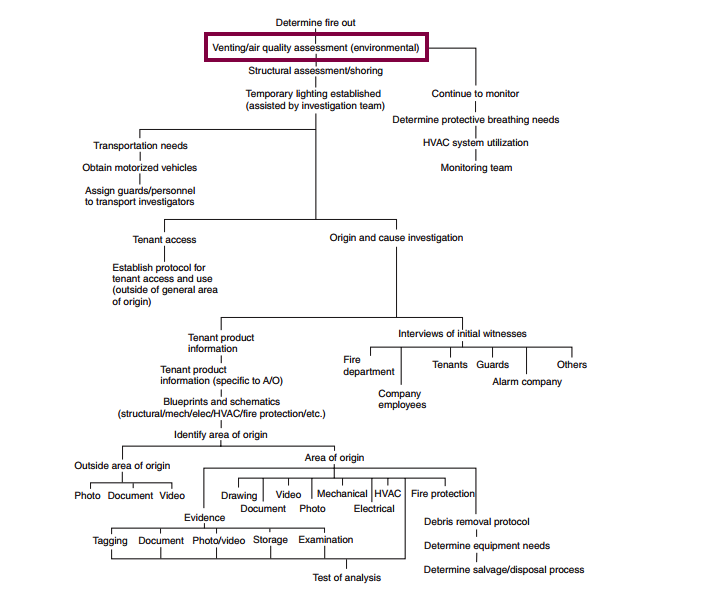
\includegraphics[scale=0.75]{flowchart.png}
\caption{Fire Investigation Flowchart  \cite{nfpa}}
\label{fig:FireInvesFlowChart}
\end{figure}

During the "Venting/air quality assessment step" in Figure ~\ref{fig:FireInvesFlowChart}, there is a sub-step that prompts the fire investigators to "determine protective breathing needs."\cite{nfpa} This is the primary focus of our vehicle's functionalities.

Currently, in order to asses the types of air quality risks within a post-fire environment (and therefore the types of protective breathing needs/clothing), a responder must enter the environment equipped with some degree of protective gear and various sensors. These sensors include, but are not limited to, multi-gas detectors and air particulate detectors.\cite{evaluationofhazards} Once the environment is assessed and the proper protective gear is chosen, the post-fire procedure can commence. Therein lies the problem. In order to assess the harmful gasses and particulates in a post-fire zone, a person must enter said zone. This person could potentially be exposed to excessive: carbon monoxide, carbon dioxide, air particulates, and toxic chemicals from the fire and fire retardants. \cite{toxichazards}


We have used the sources we have found to develop our vehicle in such a way that it can perform all of the tasks that a responder would, as well as provide additional data that can be used to further ensure that no humans will be harmed during the post-fire assessment/investigation/recovery procedure. 
Our vehicle has been equipped with multiple useful sensors that reveal air quality conditions to operators who are controlling the vehicle from a safe distance. The operators also receive a live video stream as the vehicle traverses the environment. All of the relevant information can be visualized and analyzed through our web-based user interface. 

In addition, our vehicle will generate a useful map of the environment, which is something a human who is traversing the scene cannot do on his own. This 3D map can serve as a resource for other people who will enter the post-fire environment. The operators will be able to identify "hot spots" and other notable zones. When assessing post-fire environments, it is useful to keep track of particularly hot or dense, gaseous zones in order to maximize safety for the humans involved. \cite{recoveringfromwildfire}

The sources we found have provided information on and inspiration for the exact role our vehicle can serve in aiding those who assess post-fire environment. Our vehicle will help operators determine the state of the environment and keep humans out of any particularly hazardous situations. 





\section{Problem Statement}

Our goal was to design and implement an unmanned vehicle
that gathers and relays information on potentially 
hazardous environmental conditions back to its operators.

To do this, we planned to accomplish the following:
\begin{itemize}
\item equip the Polaris 6x6 Ranger with appropriate sensors and cameras to determine how safe the environment is for humans to enter
\item use GPS and laser scans to generate a 3D map that operators can use to define certain zones as particularly dangerous.
\item incorporate partially-autonomous sensing capabilities that help the operator successfully drive the vehicle by remote control
 \end{itemize} 
 The result is a rugged, advanced vehicle that can be used to protect fire responders from any lingering hazards during the investigation of a post-fire environment. 



\section{Vehicle Background}
The vehicle was built for the 2004 and 2005 DARPA Grand Challenge competitions by a privateer team called Team Overbot \cite{rslrover2014}.  Unfortunately, the vehicle did not meet requirements for the challenge either year and was then donated to University of California Santa Cruz.  Students at UC Santa Cruz worked on the vehicle trying to expand its autonomous functions.   UC Santa Cruz then donated the vehicle to Santa Clara University for use in the Robotic Systems Laboratory.  The vehicle was in a state of disarray after being passed around for ten years.  

The vehicle is a 2004 Series 11 Polaris Ranger 6x6 \cite{rslrover2014}.  It contains a single-cylinder carbureted gasoline engine which produces approximately 40 horsepower.  The two rear axles have fixed differentials, forcing the four wheels to always turn at the same speed.  It has a rated top speed of 40 mph and the bed is a tilting unit and raises up allowing contents to be dumped out of the vehicle.  

Two previous Senior Design teams worked on the vehicle in 2014 and 2015.  The 2014 Senior Design team focused on creating an autonomous vehicle testbed.  They successfully developed a software control system to operate the vehicle via a remote console, redesigned the wiring of the vehicle, and implemented safety features.  They used Arduino microcontrollers to control steering, throttle, breaks, transmission and the parking break \cite{rslrover2014}.  All of these microcontrollers and emergency stop safety features are still present and in use in our current system.

The 2015 Senior Design team attempted to build on the system developed by the 2014 Senior Design team and add sensors and microprocessors to  give the vehicle autonomous capabilities \cite{rslrover2015}.  At the end of their year of work, the 2015 Senior Design team successfully implemented obstacle detection using a LIDAR unit.  When the vehicle detected an object in it's path, it would make an emergency stop in order to avoid collision \cite{rslrover2015}. Currently, the vehicle still houses the LIDAR unit but no longer performs obstacle detection, as we have developed our own software using the LIDAR. 

